\documentclass[]{spie}  %>>> use for US letter paper
%\documentclass[a4paper]{spie}  %>>> use this instead for A4 paper
%\documentclass[nocompress]{spie}  %>>> to avoid compression of citations

\renewcommand{\baselinestretch}{1.0} % Change to 1.65 for double spacing

\usepackage{amsmath,amsfonts,amssymb}
\usepackage{graphicx}
\usepackage[colorlinks=true, allcolors=blue]{hyperref}
% user added packages
\usepackage{xcolor}
\usepackage{adjustbox}
\usepackage{ulem}
%\usepackage{natbib}

% user added commands
\newcommand{\comr}[1]{\textcolor{red}{#1}}
\newcommand{\comb}[1]{\textcolor{blue}{#1}}
\newcommand{\dgr}{$^\circ$}

% journal abbreviations for bibtex
\def\aap{\it{A\&A}}
\def\apj{\it{ApJ}}                 % Astrophysical Journal
\def\apjl{\it{ApJ}}                % Astrophysical Journal, Letters
\def\apjs{\it{ApJS}}               % Astrophysical Journal, Supplement
\def\ao{\it{Appl.~Opt.}}           % Applied Optics


\title{Optical Design of PICO, a Concept for a Space Mission to Probe Inflation and Cosmic Origins}

\author[a\dag]{Karl Young}      %UMN
\author[b]{Marcelo Alvarez}  % University of California Berkeley, USA
\author[c]{Nicholas Battaglia}  %  Princeton
\author[d]{Jamie Bock}       % Caltech
\author[e]{Jullian Borrill}  % LBNL
\author[f]{David Chuss}  % Villanova  University, USA
\author[g]{Brendan Crill}    % JPL
\author[h]{Jacques Delabrouille}  % APC
\author[i]{Mark Devlin}  % U Penn
\author[j]{Laura Fissel}  % NRAO, USA
\author[k]{Raphael Flauger} % UC san diego 
\author[l]{Daniel Green}  % University of Toronto, Canada
\author[g]{Kris Gorksi}  % JPL
\author[a]{Shaul Hanany} % UMN
\author[m]{Richard Hills} % Cambridge
\author[n]{Johannes Hubmayr} % NIST, USA
\author[o]{Bradley Johnson}  % Columbia University, New York
\author[c]{Bill Jones}  %Princeton 
\author[p]{Lloyd Knox}  % UC Davis
\author[q]{Al Kogut}  %Goddard
\author[g]{Charles Lawrence}  % JPL
\author[r]{Tomotake Matsumura} % IPMU, Tokyo
\author[g]{Jim McGuire}  % JPL
\author[s]{Jeff McMahon}  % U of MI
\author[g]{Roger O'Brient} %JPL
\author[a]{Clem Pryke}  % UMN
\author[a]{Xin Zhi Tan}  % UMN
\author[g]{Amy Trangsrud}  % JPL
\author[a]{Qi Wen}  % UMN
\author[t]{Gianfranco de Zotti}  % padova, Osservatorio Astronomico di Padova, Italy

%Brian?

\affil[a]{University of Minnesota, USA}
\affil[b]{University of California Berkeley, USA}
\affil[d]{California Institute of Technology, USA}
\affil[e]{Lawrence Berkeley National Laboratory, USA}
\affil[f]{Villanova  University, USA}
\affil[g]{Jet Propulsion Laboratory, California Institute of Technology, USA}
\affil[h]{Laboratoire AstroParticule et Cosmologie adn CEA/DAP, France}
\affil[i]{University of Pennsylvania, USA}
\affil[j]{NRAO, USA}
\affil[k]{University of California, USA}
\affil[l]{University of Toronto, Canada}
\affil[m]{Cavendish Laboratory, University of Cambridge, UK}
\affil[n]{NIST, USA}
\affil[o]{Columbia University, USA}
\affil[c]{Princeton University, USA}
\affil[p]{University of California Davis, USA}
\affil[q]{Goddard Space Flight Center, USA}
\affil[r]{Kalvi IPMU, University of Tokyo, Japan}
\affil[s]{University of Michigan, USA}
\affil[t]{Osservatorio Astronomico di Padova, Italy}

\authorinfo{$^\dag$E-mail: kyoung@astro.umn.edu, Telephone: 1 612 626 9149}

% Option to view page numbers
\pagestyle{empty} % change to \pagestyle{plain} for page numbers   
\setcounter{page}{1} % Set start page numbering at e.g. 301
 
\begin{document} 
\maketitle

\begin{abstract}
\comr{Abstract Submitted Nov. 2017, needs polishing.}

% The Probe of Inflation and Cosmic Origins (PICO) is a probe-class mission concept currently under study by NASA.  PICO will probe the physics of the Big Bang 
% and the energy scale of inflation, constrain the sum of neutrino masses, measure the growth of structure in the universe, and constrain its reionization 
% history by making full sky maps of the cosmic microwave background with sensitivity 70 times higher than the Planck space mission. With broad frequency coverage from a tens to hundreds of GHz, PICO will make polarization maps of galactic synchrotron and dust emission, thus elucidating the role of galactic magnetic fields in the process of star formation. 

% We describe the PICO instrument, including the 1.4 meter telescope, the frequency coverage, the detector technology, and the intended survey of the sky.  We will discuss the choice of optical system, present the design of the focal plane, and give the expected noise level. 

%\comr{new abstract}

The Probe of Inflation and Cosmic Origins (PICO) is a probe-class mission concept currently under study by NASA.  PICO will probe the physics of the Big Bang 
and the energy scale of inflation, constrain the sum of neutrino masses, measure the growth of structure in the universe, and constrain its reionization 
history by making full sky maps of the cosmic microwave background with sensitivity 70 times higher than the Planck space mission. With bands at 
21-799~GHz and arcmin resolution at the highest frequencies, PICO will make polarization maps of galactic synchrotron and dust emission to observe  
the role of Galactic magnetic fields in galactic evolution and star formation. 
We describe the current state of the PICO instrument design.  We will discuss the choice of optical system, present the design of the focal plane, 
and give the expected noise level. 





\end{abstract}

% Include a list of keywords after the abstract 
\keywords{Cosmic microwave background, cosmology, mm-wave optics, polarimetry, instrument design, satellite, mission concept}



\section{INTRODUCTION}
\label{sec:intro}  

\comr{Probe study language copied directly from Brian's paper (May 6th).  What level of repeat is useful?  What is appropriate?}
\comb{Answer: you shouldn't copy the same text. Find a different way to say the same thing, or simply point people to the other paper.} 

In astronomy and astrophysics, NASA currently flies small and medium Explorer missions ($<$\$250M), as well as multi-billion-dollar flagship observatories like JWST and WFIRST. There are a number of science opportunities that are beyond the scope of the Explorer program, but don't require flagship-level funding. To explore these opportunities, NASA has funded studies of 10 `Probe' class (\$400M-\$1B) mission concepts. The Probe of Inflation and Cosmic Origins (PICO) is one of these mission studies. Reports of these mission studies are due to NASA at the end of the 2018 and NASA's plan is to forward the reports for consideration by the next Astronomy and Astrophysics Decadal panel. This paper comes part way through the PICO study, and describes a snapshot of the  instrument design at this time in the study.

Astrophysical observations in the  millimeter and sub-millimeter region of the electromagnetic spectrum contain a wealth of 
information about the formation, evolution, and structure of the Universe.  
\comb{new:} The polarization and temperature anisotropy of the of the cosmic microwave 
background (CMB) encode fundamental physics information relating to  the epoch of inflation, to the mass of the neutrinos,  
and to the number of relic light particles in the early Universe. They also contain information about the formation of 
the first stars, galaxies, and clusters.  Information about the role of magnetic fields in star formation and galactic evolution is obtainable 
by observing the polarized emission of Galactic dust, which 
traces magnetic fields, at high resolution. Targeting both of these regimes, PICO will survey the entire sky with 
unprecedented polarization sensitivity 
in 21 bands centered at 21--799~GHz.  Details of these science targets and expected constraints from PICO 
are in a companion paper, Sutin~et~al.\cite{brian_spie} 
In this paper we discuss the mission's optical system, focal plane, and sensitivity.


\comb{old: Large scale cosmological and fundamental 
physics information, such as 
evidence of inflation, the effect of the first stars and galaxies, constraints on neutrino masses, and limits on light particles beyond 
the standard model, is contained in the temperature and polarization anisotropies of the cosmic microwave 
background (CMB). } 

% %(check LB's intro?, although I probably won't like that.)

\section{SPACECRAFT AND MISSION}
\label{sec:spacecraft}

%  This could all be in the intro instead. Purpose is to show constraints on the optics to motivate decisions discussed later.  

The PICO will conduct scientific observations for five years from the Earth-Sun L2 Lagrange point. The spacecraft design impacts 
the optical design and sensitivity in two primary ways; volume constraints limit the physical size of the telescope and optical component 
temperatures impact noise levels.  

The maximum size of the spacecraft is limited by the launch vehicle, SpaceX's Falcon 9, which carries payloads up to 4.6~m in diameter. 
This diameter limit sets the V-groove size which, along with the scan strategy, defines the `shadow cone' in Figure~\ref{fig:cad}.  
The shadow cone is the volume protected from solar illumination, and all optical components must remain within it. The shadow cone and 
inner V-grooves define an available volume for the telescope.  

The temperatures of all optical elements are given in Figure~\ref{fig:cad} \comb{see comment in caption in regard to the temperature 
of the primary. Check with Paine}.  The optics box, secondary, and focal plane are actively cooled, 
details of the thermal system are given in Sutin~et~al.\cite{brian_spie}. \comb{looks like the primary is also actively 
cooled. check with Paine.}

\begin{figure} [ht]
\begin{center}
%\begin{tabular}{c} %% tabular useful for creating an array of images 
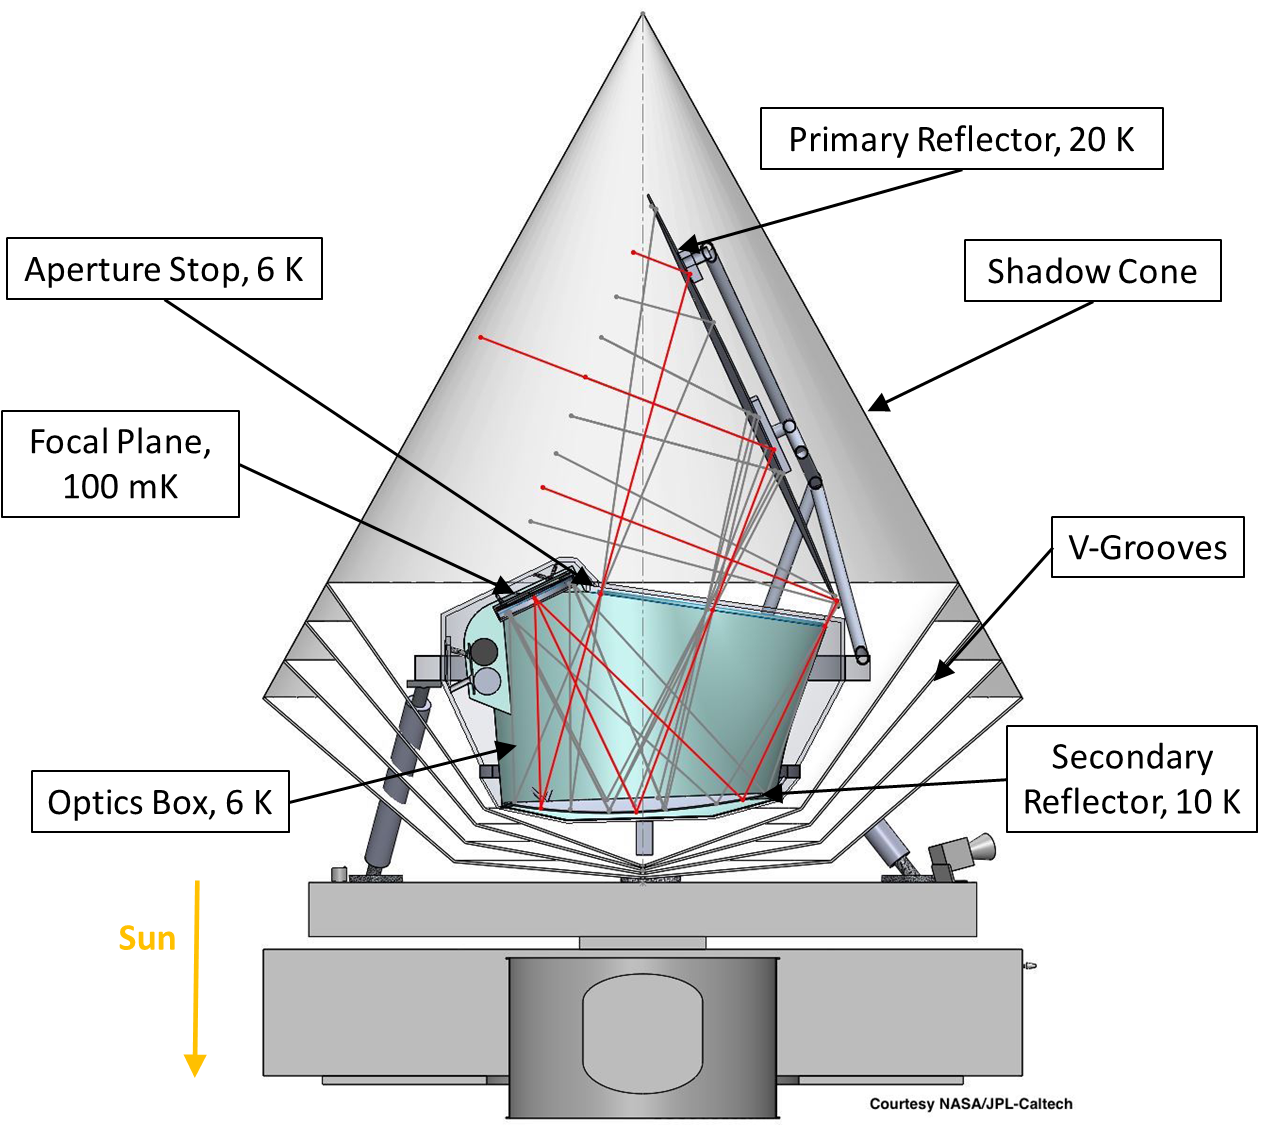
\includegraphics[height=9cm]{PICO_CAD_annotated.png}
%\end{tabular}
\end{center}
\caption { \label{fig:cad} 
Mechanical design of the PICO satellite. Components relevant to this paper are labeled, for other details see Sutin~et~al.\cite{brian_spie}
\comb{is the primary really at 15 K? hard to believe. Need to verify. To explain the idea of a 'shadow cone', need to say something 
about where the Sun is and how it illuminate the spacecraft such as to give this 'shadow cone'. } 
}
\end{figure} 

% \begin{itemize}
% \item Sketch out satellite systems. Include CAD model figure and table of system parameters
% \subitem thermal systems and surface temperatures (NOTE! a bunch of these in Brian's paper don't match what we have used.  filters 1 K, stop 4.5-6 K, secondary 10 K, Primary 20 K, maybe others. Unclear how much of this will be in final version.
% \subitem sunshields and scan strategy
% \subitem observing frequency ranges 
% \item Summarize mission 
% \subitem L2 orbit, for earth-moon viewing angles
% \subitem 5 yrs active time frame
% \subitem launch vehicle is Falcon 9 
% \end{itemize}

% \vspace{4in}

\section{OPTICAL SYSTEM}
\label{sec:optics}

The PICO telescope is a 1.4~m \comb{aperture} modified open-Dragone.  This choice was driven by a combination of science
requirements and the physical limits discussed in Section~\ref{sec:spacecraft}.  The science requirements are: a large diffraction 
limited field of view (DLFOV) sufficient to support $\mathcal{O}(10^4)$ detectors, arcminute resolution at 800~GHz, low 
instrumental polarization, and low sidelobe response. Additionally, 
the transition edge sensor bolometers baselined for PICO require a telecentric focal plane which is sufficiently flat that it 
can be tiled by 10~cm detector wafers without reduction in optical quality. \comb{More than 30 years ago Dragone analyzed the 
performance of several off-axis systems and found solutions that give low cross-polarization at the center of the field 
of view, and that cancel astigmatis, or astigmatism \it{and} coma to first order}\cite{dragone}\comr{is that correct? give more references}.  
\comb{A number of recent CMB instruments used off-axis systems, and several 
began the design optimization with systems based on designs by
Dragone\cite{planck2000_optics,ACT2011_optics,SPT2008_optics,core2018_inst,LB2016_optics}. For PICO we began 
the optimization with a Dragone system that to our knowledge hasn't yet been implemented before. 
We call it `0pen-Dragone' because of its overall geometry, see Figure~\ref{fig:ray}, and as contrast to the widely 
used `cross-Dragone'. }

\comr{An advantage of the open-Dragone system relative to the cross-Dragone is that it is easier to baffle the focal plane
and thus to eliminate side-lobes. An advantage relative to a Gregorian design is that it has larger DLFOV. Our studies 
indicate however that for the same aperture size and focal length, a cross system has a DLFOV that is $\sim$1.3 times 
larger than the open. CHECK. 1.1? 1.2? 1.3?}

We design the initial open Dragone following Granet's method\cite{granet2001}. 
We find a solution \comr{with the largest aperture that still satisfies the volume constraints and has a large 
DLFOV}\comb{what about focal length?}.  We force a circular aperture stop 
between the primary and secondary mirrors and numerically optimize its angle and position to obtain the best 
optical performance.  The stop diameter provides an effective 1.4~m aperture on the primary for the center feed.  
Adding a stop in this way increases the size of the primary mirror, \comb{as} the primary is unevenly illuminated at various 
field angles \comr{karl, if you want to start a new sentence without using a period, please use a semi colon, not a comma. Generally, 
however, it is best to stick to simple grammatical structures}. 
Actively cooling the aperture stop, however, reduces detector noise, and the stop shields the 
focal plane from stray radiation. At this stage the system still meets 
the Dragone condition and is defined by the `Initial Open Dragone' parameters in Table~\ref{tab:optics}.

\comb{In his publications Dragone provided a prescription to eliminate coma
in addition to the cancellation of astimgatism, which is provided by the baseline designs.} The reflector corrections 
call for adding distortions of the primary and secondary reflectors, 
which scale as $r^4$ where $r=0$ is at the chief ray impact point on each mirror \comr{is that true?}. 
We thus attempted to increase the DLFOV using two methods. 

In the first method, one of the coauthors (RH) used Zemax and added Zernike 
polynomials which were offset by $h=624.2$~cm for the primary and $76.1$~cm for the secondary.  
This places \comr{mix of tenses. present tense or past tense?} the origin of polynomials at the 
chief ray impact point for each mirror. \comr{what do you mean 'offset by $h$'? has $h$ been defined?}
Inspired by the Dragone corrections, all Zernike terms up to fourth order and the first fifth order term were allowed to vary. 
The optimization metric was minimization of the rms spot \comb{size; what does 'size' mean?} diameter at 
the following locations: the center of the FOV, $\pm2$\dgr\ in Y, and $\pm4$\dgr\ in X. The center of the FOV was 
most heavily weighted \comr{what was the relative weighting?}. To constrain the optimization, the X and Y 
effective focal lengths are held fixed as is the impact point of the chief ray on the focal plane. 

This optimization step increases \comr{tenses!} the \comr{DLFOV}
by 15\% at 21~GHz, by 2.4$\times$ at 155~GHz, and by 
10.5$\times$ at 799~GHz. \comr{is this proper English? 2.4$times$? I don't think so. Why change between \% and $\times$?} 
We improve the system further by allowing the focal plane radius of 
curvature to vary \comr{if it has a radius of curvature, please call it focal surface} and rerunning the optimization.  
This gives a 50\% increase in diffraction limited area at all frequencies over the Zernike polynomials alone.  
Finally, an approximately 4\% additional gain in area can be achieved by adding Zernike terms 
up to sixth order, allowing the secondary to focal plane distance to vary, adding a weighted constraint on the effective focal length, 
and adding fields with low weight to the rms spot diameter metric at $\pm7.5$\dgr\ in Y and $+15$\dgr\ in X, 
without these additional fields the 
corrections at the mirror edges are not well constrained \comr{again, a sentence on its own, separated only by coma}.

\comr{The other method by Richard has the first step of converting the conics into an on axis XY polynomial respresentation. Then the same procedure is followed.  It is less well behaved during optimization.  This second Richard method is what I replicated in CodeV.}
\comb{is this 'other method' = method2? or is it 1b?}



\begin{figure} [ht]
\begin{center}
%\begin{tabular}{c} %% tabular useful for creating an array of images 
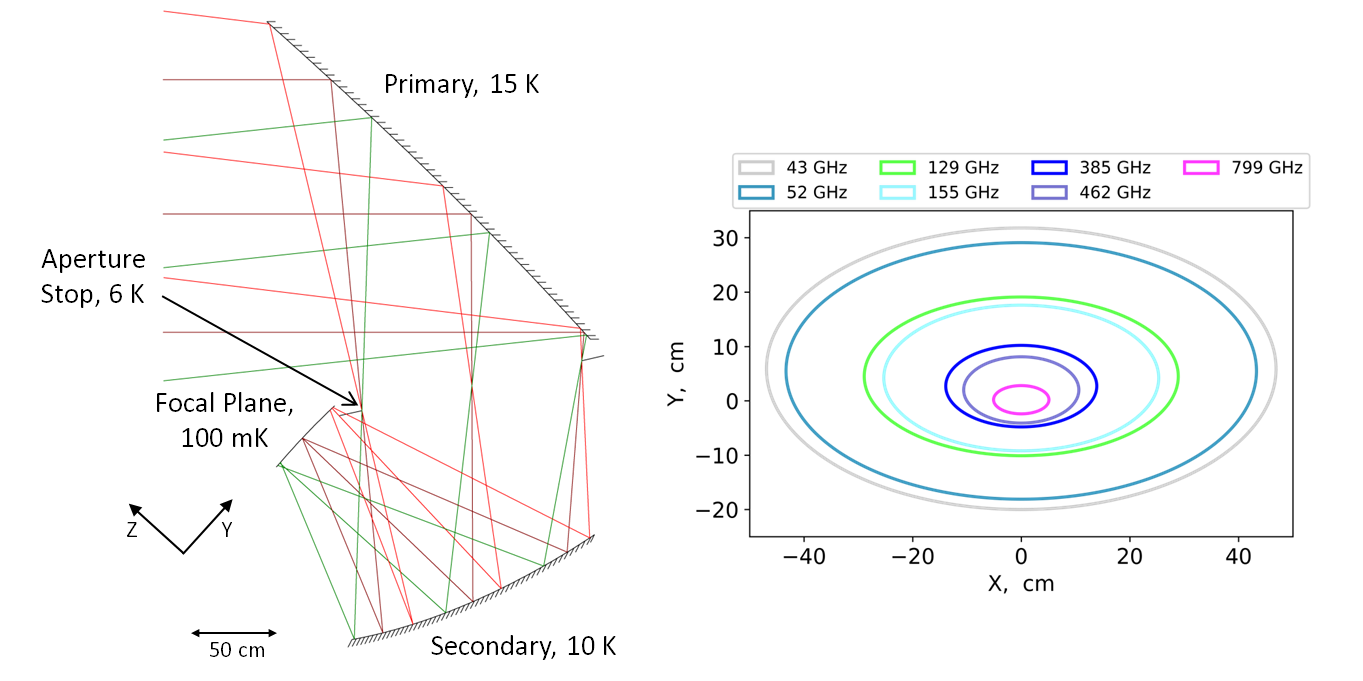
\includegraphics[height=7.5cm]{jpl_ray_strehl.png}
%\end{tabular}
\end{center}
\caption { \label{fig:ray} \label{fig:strehl} 
Raytrace (left) and Strehl~$=0.8$ contours (right) for the PICO optical design.
}
\end{figure} 

\begin{table}[ht]
\centering
\caption{Telescope geometric parameters  \label{tab:optics}}

\begin{adjustbox}{width=1.05\textwidth}
\hspace{-1cm}
\begin{tabular}{|l|llll||ll|}
\hline
\multicolumn{5}{|c||}{PICO optical system}                                    & \multicolumn{2}{c|}{Initial Open Dragone$^b$}     \\ \hline
                          & Primary           & Secondary    & \multicolumn{2}{c||}{Telescope parameters$^b$} & \multicolumn{2}{c|}{Fundamental design parameters}  \\
Mirror size$^a$ (cm)      & $270 \times 205$ & $160 \times 158$ & Aperture (cm)           & 140      & Aperture (cm)                  & 140   \\
Radius of curvature (cm)  & $\infty$         & 136.6             & Focal ratio, F             & 1.42     & $\theta_0$ (degrees)           & 90    \\
Conic constant, $k$       & 0                 & -0.926            & h (cm)                    & 624.2    & $\theta_e$ (degrees)           & 20    \\
Normalization radius (cm) & 524.8             & 194.1             & $\alpha$ (deg)            & 74.2     & $\theta_p$ (degrees)           & 140   \\
4th Zernike Coefficient   & 2018.4            & -61.1             & $\beta$  (deg)            &  62.3    & L$_m$ (cm)                     & 240   \\
9th Zernike Coefficient   & -37.0             & 16.7              & L$_m$ (cm)                &   229.3  &                                &         \\
10th Zernike Coefficient  & -2919.8           & -15.1             & L$_s$ (cm)                &   140.5  & \multicolumn{2}{c|}{Derived parameters} \\ 
11th Zernike Coefficient  & -1292.7           & 22.3              &                           &          & Focal ratio, F                 & 1.42  \\   
12th Zernike Coefficient  & 120.6             & -3.8              &   \multicolumn{2}{c||}{Focal Plane}  & h (cm)                         & 624.2 \\   
13th Zernike Coefficient  & -74.5             & 4.9               & Diameter (cm)             & 69 x 45  & $\alpha$ (deg)                 & 38.6  \\   
19th Zernike Coefficient  & -75.8             & 3.4               & Diameter (deg)            & 19 x 13  & $\beta$  (deg)                 & 101.4 \\   
20th Zernike Coefficient  & -398.9            & 6.3               & Radius of curvature (cm)  & 455      & L$_s$ (cm)                     & 122.2 \\   
21st Zernike Coefficient  & -319.5            & 23.3              &                           &          & Primary, $f$ (cm)              & 312.1 \\   
22nd Zernike Coefficient  & -276.6            & -8.5              &                           &          & Secondary, $a$ (cm)            & 131   \\   
23rd Zernike Coefficient  & -201.6            & -3.2              &                           &          & Secondary, $e$                 &  1.802  \\
24th Zernike Coefficient  & -127.4            & -1.9              &                           &          &                                &       \\
25th Zernike Coefficient  & -55.0             & 0.1               &                           &          &                                &       \\\hline
\multicolumn{7}{l}{\footnotesize  $^a$ The maximum physical size of the mirrors.}\\
\multicolumn{7}{l}{\footnotesize  $^b$ Telescope parameters follow the definitions in Granet 2001.\cite{granet2001}} \\
%\multicolumn{7}{l}{\footnotesize  $^b$ } \\
\end{tabular}
\end{adjustbox}
\end{table}

%To increase the optical performance we use CodeV to numerically optimize the system.  
In the second optimization method, another coauthor (JM) used CodeV and allowed more of the geometric 
parameters of the system to vary.  To adjust the 
mirror shapes, we add \comr{tenses} a low order \comr{what does 'low order' mean?}, 4th and 9th-13th, 
Zernike polynomial correction to each conic surface \comr{what do you mean 'each'? more than two?}. 
The Zernike polynomials are defined on the same coordinates as the base conics.  We allow the focal plane curvature 
and focal plane to secondary distance L$_s$ to vary.  The primary-secondary distance L$_m$, primary offset $h$, 
and the primary and secondary rotation angles, $\alpha$ and $\beta$, are varied as well.  The optimization 
metric is the rms spot size \comr{diameter} across the field of view, with additional weighted constraints requiring telecentricity and 
maintaining the x- and y-focal lengths \comr{capital X,Y or small x,y?}.  We also added Lagrange constraints 
to enforce beam clearances and place an upper limit on overall system size.  Once the optimization converged to 
an acceptable optical system, we added the higher order Zernike terms, 19th-25th, and refined t
he mirror shapes using the same metric and constraints. \comr{please find a better way 
to express the parameters varied without so many also's.}
The current PICO optical design is from this optimization procedure.


Figure~\ref{fig:compare} 
%we show the final optimized system compared with the `Initial Open Dragone' and give the Strehl~$=0.8$ contours.  One sees 
shows that the optimization reduces the overall telescope volume, allowing it to fit more easily within the shadow cone, 
and increases the DLFOV.  
The DLFOV increases by 1.9$\times$ at 21~GHz and by 4.6$\times$ at 799~GHZ. \comr{This is relative to which 
baseline? need to provide improvement relative to the same starting point, but also give improvement relative 
to method1.}
The most important gain in the DLFOV is at 129 and 155~GHz where it increased by 3.8$\times$ and 4.3$\times$, respectively.  
This added area allows us to add `C' and `D' pixels \comr{what pixels? what is C, D?} which are critical to meeting PICO's 
cosmology and fundamental physics science goals, because they contain the bands most sensitive to the CMB. Being able to 
pack 100's of `C' and `D' pixels into the focal plane is what allows PICO to reach unprecedented levels of CMB sensitivity. \comr{do 
you mean 'if we had only optimization method1 we wouldn't reach our goals?}

The geometric parameters of the PICO optical system are given in Table~\ref{tab:optics}. The 
system is diffraction limited, Strehl greater than 0.8, at the center of the field of view for 799~GHz and has a 
DLFOV of 82.4~deg$^2$ at 155~GHz \comr{This sentence is not passing English grammar scrutiny. 
Please revise. Give the total throughput}.  Strehl of 0.8 contours for all pixel types are shown in Figure~\ref{fig:strehl}. 
\comb{make sentence active voice.} 
The slightly \comb{concave, focal surface, which has a radius of curvature of 4.55~m,} is telecentric to 
within 0.12\dgr\ across the entire area.

\begin{figure} [ht]
\begin{center}
%\begin{tabular}{c} %% tabular useful for creating an array of images 
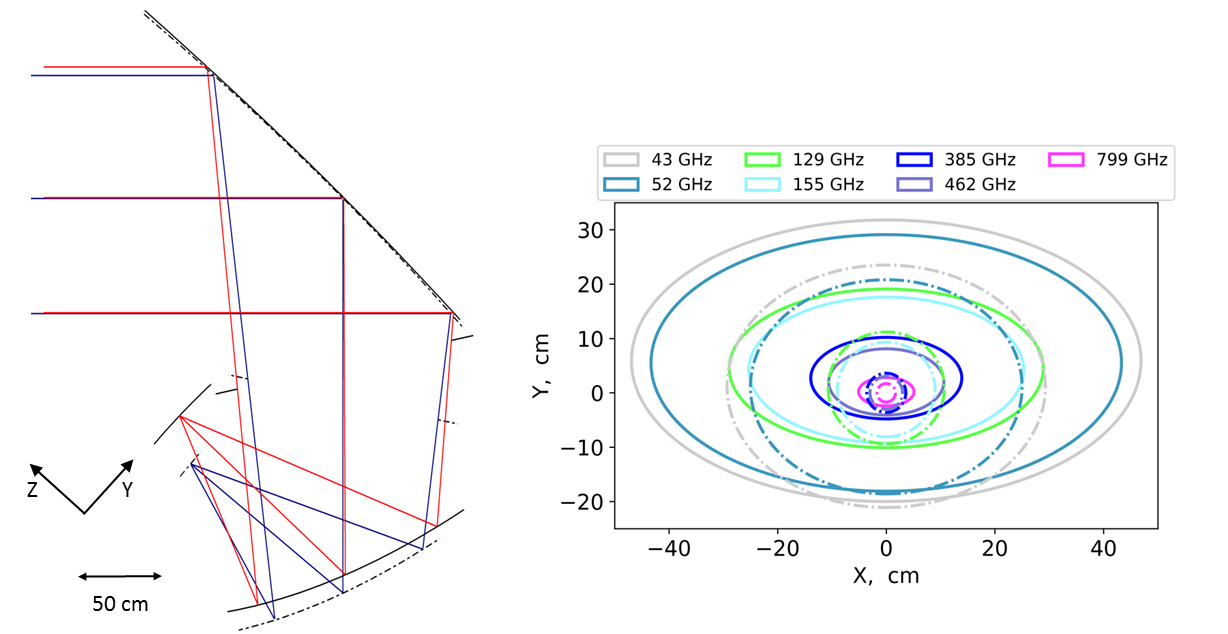
\includegraphics[height=7cm]{jpl_vs_V3D.png}
%\end{tabular}
\end{center}
\caption { \label{fig:compare} 
Comparison between optimized \comr{optimized in which way?} and unoptimized Open Dragone systems.  
The ray traces (left) are aligned at the chief ray impact point on the primary. 
The optimized system (red rays, solid mirrors) is smaller in the vertical direction \sout{and has a 
slightly flatter primary than the unoptimized version} \comb{can not see; remove} 
(blue rays, dash-dot mirrors). The overlaid Strehl~$=0.8$ contours (right) show the improvement at 
all frequencies in the optimized (solid lines) system over the unoptimized (dash-dot lines) system. 
}
\end{figure} 

An additional benefit of the optimization is the concave focal plane. The Open Dragone's focal surface is naturally curved, so matching this 
curvature reduces defocus and increases the DLFOV as well as increasing telecentricity.  The unoptimized system is telecentric to within 
2.5\dgr while the optimized version is telecentric to within 0.12\dgr. If the focal plane is too strongly curved tiling it with flat detector 
wafers would result in large defocus at the edges of these wafers.  This is not the case for PICO. The focal plane radius of curvature, 4.55~m, 
results in a defocus of 0.1~mm for the edge of a 10~cm wafer. 

%these are unoptimized comparisons. note that.

\comr{This is an important paragraph. I started making comments along these lines earlier. Need to move the paragraph 
earlier to motivate the use of the Open system.}
We considered two additional Dragone systems; a Gregorian Dragone like that used for \textit{Planck} and a Crossed Dragone 
similar to that planned for CORE or LiteBIRD \comb{I don't think Planck is formally a Dragone system; nothing is 
really 'planned' for CORE, as it is not in development}.  With half the diffraciton limited focal plane \comb{plane or surface?} 
area of the Open Dragone,\cite{core2018_inst}  the Gregorian Dragone is 
unable to support $\mathcal{O}(10^4)$ detectors, so was rejected.  
The Crossed Dragone has roughly $4\times$ the diffraction limited focal plane area of the Open \comr{is that true? I didn't 
think it was that much of a difference}, but it has well 
known issues with sidelobes \comr{not well phrased} as shown in Figure~\ref{fig:sidelobes} and always has a larger F-number 
than the Open system \comr{why does it 'always' have larger F? Can make a smaller F, no?}.  
The larger F-number results in a larger telescope that fits poorly into the shadow cone. The largest Crossed Dragone 
that meets the PICO volume contraints has 
a 1.2~m aperture while the largest Open Dragone is 1.4~m. The large F-number of the Crossed system also increases 
the physical focal plane size, and therefore mass and cost, for a fixed number of pixels.  
These disadvantages, and the success of the optimized 
Open Dragone, led us to the final PICO optical system detailed in Table~\ref{tab:optics} and shown in Figure~\ref{fig:ray}.


\begin{figure} [ht]
\begin{center}
%\begin{tabular}{c} %% tabular useful for creating an array of images 
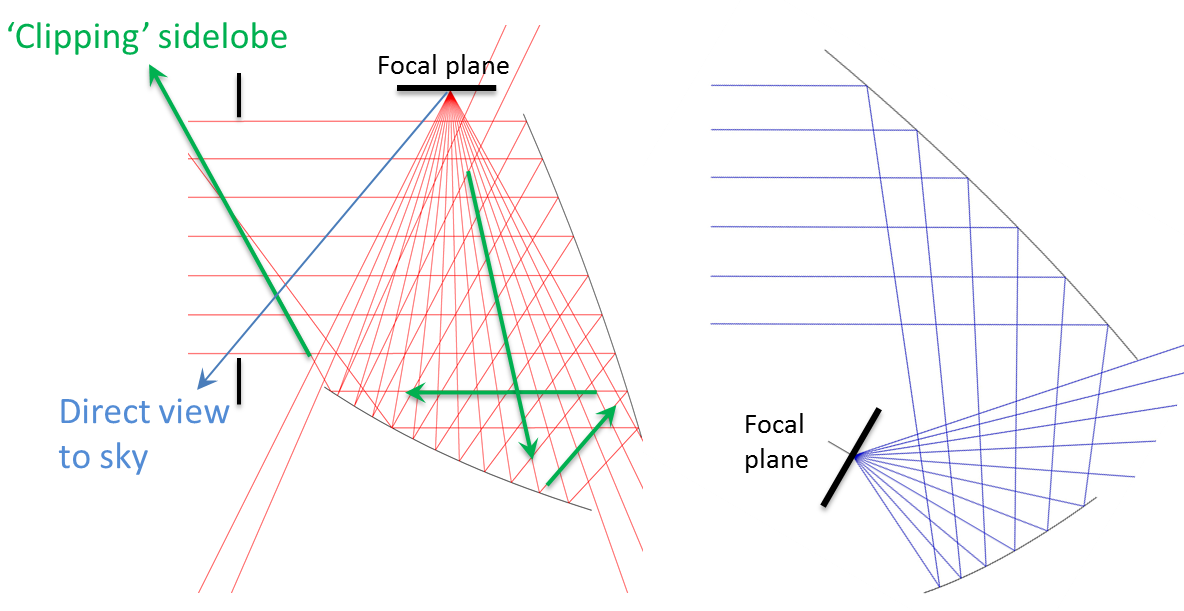
\includegraphics[height=6.5cm]{sidelobes.png}
%\end{tabular}
\end{center}
\caption { \label{fig:sidelobes} 
Comparison of sidelobes for typicalexample Crossed (left) and Open (right) Dragones.  Rays are traced from the center of the focal plane toward the sky.
For both systems spillover around the secondary is straightforward to mitigate with absorptive baffles.  However, the sidelobe and direct 
sky view in the Crossed system require a long forebaffle or large F-number to mitigate, both of which are problematic in the PICO case.}
\end{figure} 


%
%Grasp? maybe.  Beam and sidelobe would be pleasent.
%

\section{FOCAL PLANE}
\label{sec:focalplane}

Modern mm/sub-mm detectors are photon noise limited, so the primary way to increase sensitivity is to increase the number of detectors. 
The PICO focal plane has 12,996 detectors, $175\times$ the number flown on \textit{Planck}. PICO achieves this by having a large DLFOV and using 
multichroic pixels (MCPs)\cite{Suzuki2014_samps}.  
%Multichroic pixels are a recent mm-wave pixel technology made up of a broad-bandwidth 
%polarization sensitive antenna lithographed onto a silicon substrate which couples to microstrip transmission lines to carry the signal 
%to a channelizing filter. The filter divides the broadband signal into individual bands and 
%directs it to separate transition edge sensor (TES) bolometers. 
The MCP architecture assumed for PICO has three bands per pixel with two single polarization transition 
edge sensor (TES) bolometers bolometers per band and therefore six bolometers total. 
We assume the MCPs are coupled to free space using lenslets\cite{Suzuki2014_samps}, however the pixel size, number, and spacing is 
relatively agnostic to the coupling scheme, so the current layout would not change significantly if horn or phased array coupling was used 
instead.

We design PICO with 21 overlapping bands centered at 21--799~GHz and divided amongst nine pixel types, A-I; see Figure~\ref{fig:bands}. 
These bands provide the broad fequency coverage needed to seperate the CMB, Galactic dust, and various foregrounds using their differing spectra.  
%The PICO bands are logarithmically spaced with 25\% fractional bandwidth.  
The 25\% fractional bandwidth is broader than the interband spacing, so the neighboring bands overlap and must be in separate pixels.  
For example, bands 1, 3, and 5 are in pixel A while bands 2, 4, and 6 are in pixel B.  This 
complicates the pixel design and focal plane layout, but allows broader bands to increase total sensitivity.  

\begin{figure} [ht]
\begin{center}
%\begin{tabular}{c} %% tabular useful for creating an array of images 
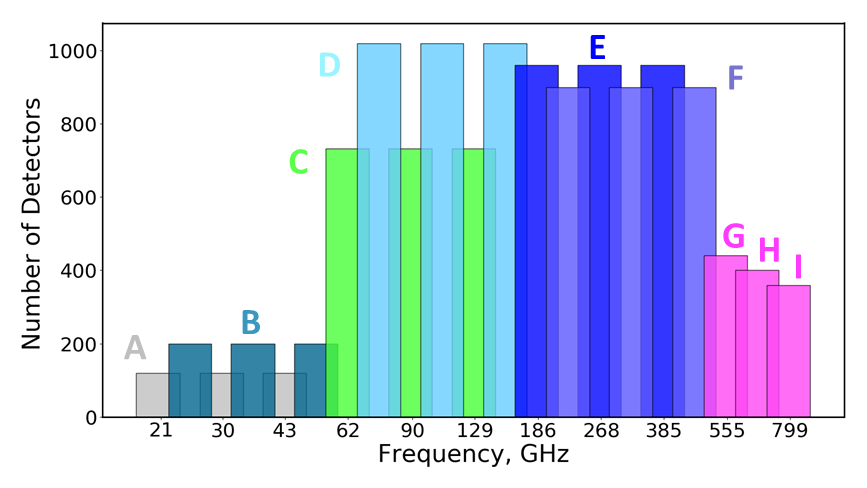
\includegraphics[height=6cm]{bands_label.png}
%\end{tabular}
\end{center}
\caption { \label{fig:bands} 
Frequency coverage of the PICO bands. Each color (excluding magenta) denotes a different MCP, labeled A-F. The bar height 
indicates the number of detectors per band.  Width gives the bandwidth, all are top-hats with 
25\% fractional bandwidth; the $x$-axis is logarithmic.  The three highest frequencies (magenta) are single color pixels G, H, I.
}
\end{figure} 

The exceptions to this MCP architecture are the highest three bands.  These three bands are above the superconducting band gap of niobium, so 
the niobium transmission lines and filters used in MCPs are unsuitable.  Instead we will use polarization sensitive, feedhorn 
coupled bolometers at these frequencies, similar to the \textit{Planck}\cite{planck2010_hfi} or Herschel SPIRE\cite{spire2010} detectors.  

The PICO focal plane is designed to take maximum advantage of the large field of view.  The optical quality peaks at the 
focal plane center and falls off with radius as shown in Figure~\ref{fig:strehl}.  This pattern dictates the layout shown 
in Figure~\ref{fig:focal_plane}. The highest frequency pixels are centered on the focal plane and low frequency pixels are arranged 
around the edge. The maximum radial distance for a given pixel is the point where 
the Strehl ratio for the upper edge of the highest frequency band within that pixel equals 0.8.  Interior to these contours, the ellipses in 
Figure~\ref{fig:focal_plane}, the Strehl ratio increases ensuring pixels are diffraction limited.

\begin{figure} [ht]
\begin{center}
%\begin{tabular}{c} %% tabular useful for creating an array of images 
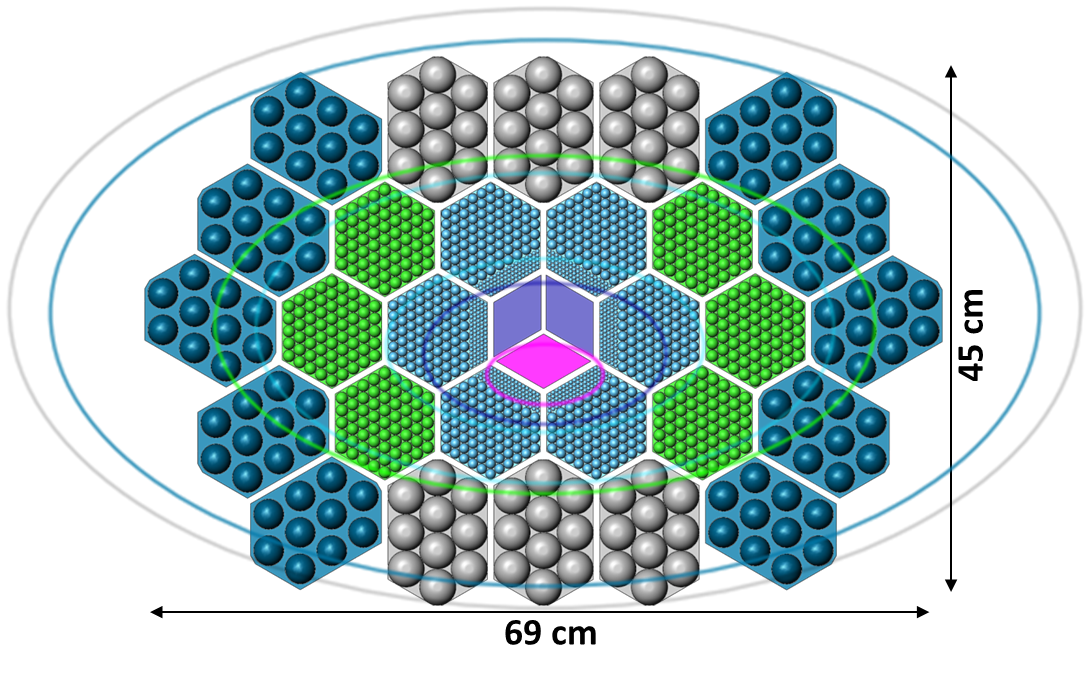
\includegraphics[height=7.5cm]{version3_focal_plane.png}
%\end{tabular}
\end{center}
\caption { \label{fig:focal_plane} 
PICO focal plane layout with Strehl~$=0.8$ contours for each pixel type. The pixel and Strehl contour colors match the band colors, A-I, 
in Figure~\ref{fig:bands} }
\end{figure} 

Optimizing the pixel size is a balance between the total number of pixels, $N_{px}$, and the efficiency with which they couple to the telescope. 
Smaller pixels pack more densely on the focal plane, $N_{px}\propto 1/D_{px}^2$, but over illuminate the stop which reduces optical efficiency 
and adds optical load.  
%Since PICO has a cold stop additional load is minimized, reducing the penalty for smaller pixels.  
We choose a pixel diameter of $2.1$F$\lambda_{mid}$, where $\lambda_{mid}$ refers to the center 
band of each pixel. This gives an edge taper, $T_e$, on the stop of 10~dB for the center band. 
Due to the multichroic nature of the pixels $T_e$ varies with band, details in Section~\ref{sec:noise}. 
We hex-pack pixels onto 94~mm hexagonal wafers to minimize wasted space for the mid-frequency pixels. 
The three central wafers have the same 94~mm hexagon footprint but are split into 
3 rhombi, shown in Figure~\ref{fig:focal_plane}, because the highest frequency magenta wafer will use different 
detector technology and will need to be fabricated separately.  

% order 0.5 sec is longer than the sample time even at 1 deg beams. sweeping 1 deg takes 0.2 sec.
The polarization sensitive bolometers in each MCP are oriented perpindicular to each other. Differencing the bolometers allows each pixel to measure Stokes Q or, if the 
pixel is rotated by 45\dgr, Stokes U. We rotate neighboring pixels which scan over the same sky location by 45\dgr, as shown in Figure~\ref{fig:QU}.
This layout reduces systematic errors by maximizing the number of Q,U pixel pairs which have almost identical optical paths and measure sky locations 
as close to simultaneously as possible.  % 'should reduce' haven't actually done these simulations . . . 
%The small time difference between Q,U measurements reduces systematic errors relating slow to drifts in detector response or 
%other 1/f noise. The proximity of the Q,U pixels also reduces errors arising from differnent telescope beam shapes and temperature gradients on the focal plane.
%\comr{Discuss Q/U orientation?}

\begin{figure} [ht]
\begin{center}
%\begin{tabular}{c} %% tabular useful for creating an array of images 
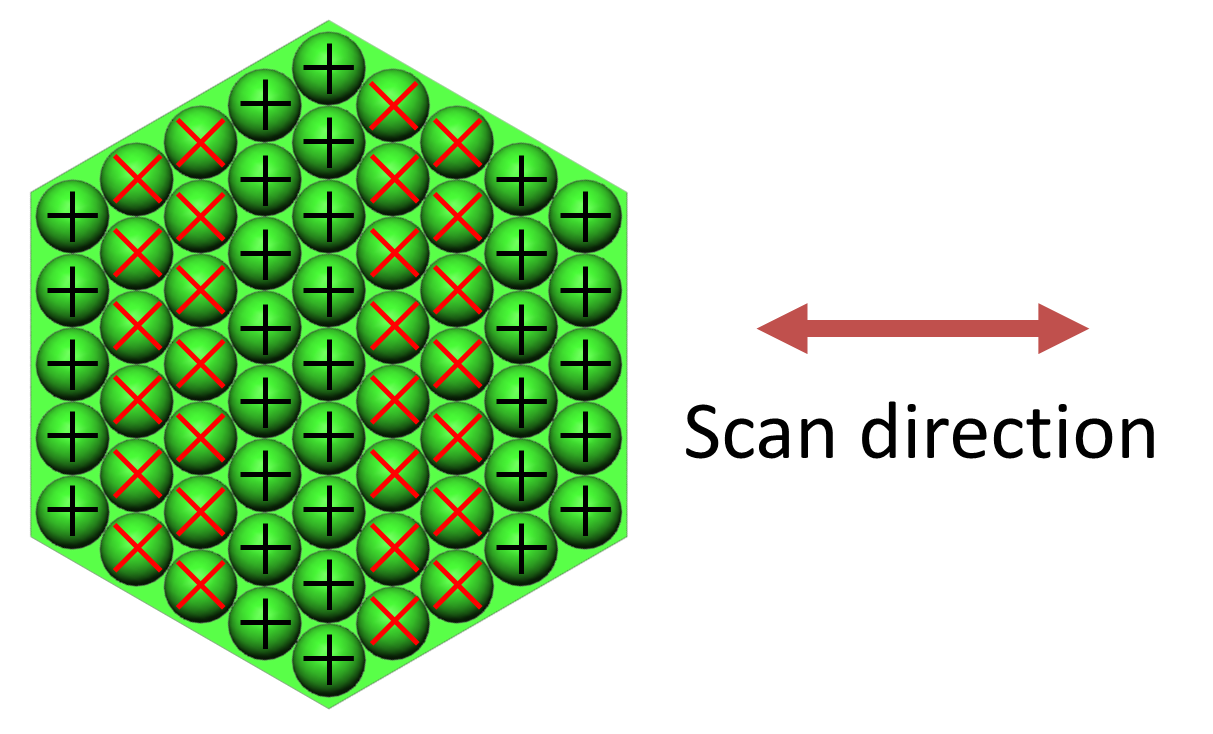
\includegraphics[height=4cm]{QU_wafer.png}
%\end{tabular}
\end{center}
\caption { \label{fig:QU} 
Layout of pixels sensitive to Stokes Q (black crosses) and Stokes U (red exes) for an example wafer.}
\end{figure}

Reading out 12,996 TES bolometers requires significant multiplexing.  Time domain (TDM) and frequency domain (FDM) 
multiplexing were explored for PICO, tradeoff details are in Sutin et~al.\cite{brian_spie}  %Ref.~\citenum{brian_spie}.  
The current PICO baseline is TDM, 
but the choice is not a driver for the focal plane layout or noise discussed in this paper.


%comment about area?

%realtive number . . . largest area by 100s. driven by science . . .

%For PICO the highest sensitivity is needed around 220~GHz, near the peak of the CMB anisotropy signal, because the inflationary signal is extremely faint.  


% \begin{itemize}
% \item Bands and multichroic pixels
% \item availible areas for pixels, focal plane layout
% \subitem Q/U orientations
% \item edge taper choices (cold stop and resolution tradeoffs)
% \subitem cold stop allows higher edge taper value. This means lower effeciency and small on-sky beam.
% \subitem edge taper varies with band due to MCPs
% \item technology types assumed for this study
% \subitem SAMPS, TES bolos, TDM readout
% \item for readout cite Brian's paper. -- description there is less comprehensive than roger's first version. May need some detail here.
% \subitem \comr{Do we want wafer level CAD sketch of cold readout? Probably too much detail for here.}
% \end{itemize}



\section{INSTRUMENT NOISE}
\label{sec:noise}
%\comr{comment somewhere in this section that these noise numbers are CBE. no margins.}

We develope an end to end white noise model of the PICO instrument to predict full mission sensitivity and 
provide a metric by which to evaluate optical, mechanical, and mission design tradeoffs.  This model does not include 
1/f noise or estimates of possible systematic effects.  %We assume TES bolometers read out using time domain multiplexing (TDM). 
%To simplify the model, we assume TES bolometers as the detector at all frequencies, even though other technologies may be better suited to the lowest bands.  
%Any suitable technology will be photon noise dominated as the TESs are, so total noise levels in the lowest bands should be relatively unaffected by 
%the use of a different detector technology.
To construct the model we follow the standard process\cite{suzuki2013_thesis,aubin2013_thesis} of estimating the 
optical load, calculating properties of the TES bolometers, calculating noise equivalent power (NEP) by source, 
combining all NEP terms to get detector noise, and finally combining all detectors to get full mission sensitivity.  
Each of these steps includes various assumptions and design decisions, 
which are discussed in this section.  The assumptions are summarized in Table~\ref{tab:assume}.
% comment on photon dominated?

\begin{table}[ht]
\centering
\caption{Noise model assumptions, see text for details. }%\comr{listing still in flux}}
\label{tab:assume}
%
\begin{tabular}{|l|l|}
\hline
%                                 &                                                  \\
Throughput                       & single moded, $\lambda^2$          \\
Fractional Bandwidth             & 25\%                                             \\
Mirror emissivity                & $\epsilon = \epsilon_0\sqrt{\nu/\text{150~GHz}}, \epsilon_0 = 0.07\%$ \\
Aperture stop emissivity         & 1                                                \\
Low pass filter reflection loss  & 8\%                                                \\
Low pass filter absorption loss$^a$  & frequency dependent, 0.2\%--2.8\%             \\
Bolometer absorption efficiency  & 70\%                                             \\
T$_e$, middle band in pixel (dB) & 10                                               \\
Bose noise fraction, $\xi$       & 1                                                \\
Bolometer yield                 & 100\%                                            \\
Bath temperature, $T_o$ (mK)    & 100                                              \\
TES critical temperature, $T_c$ (mK)   & 187                                              \\
Safety factor, P$_{sat}$/P$_{abs}$      & 2                                                \\
Thermal power law index, $n$    & 2                                                \\
Intrinsic SQUID noise (aW/$\sqrt{\text{Hz}}$)   & 3                        \\
TES operating resistance, $\Omega$    &  0.03                               \\
TES transition slope, $\alpha$    & 100                                         \\
TES loop gain                    & 14                                \\
Mission length (years)           & 5                                                \\
Observing efficiency             & 95\%                                             \\
%Multiplexing factor              &
%Number of rows/columns/whichever matters . .. 
%\comr{other?}                    &                                                  \\
\hline
\multicolumn{2}{l}{\footnotesize $^a$Assumes seperate metal mesh in polypropylene filters for each wafer.}
\end{tabular}
\end{table}


\subsection{Single bolometer noise}
\label{sec:det_noise}

\subsubsection{Model}

The sources of optical load are the CMB, primary and secondary mirrors, aperture stop, and a low pass optical filter.  These elements 
are shown schematically in Figure~\ref{fig:load}. 
%We assume the primary is 15~K, the stop 6and secondary 4~K, and the low pass filter 100~mK. % for details of the thermal design see \citenum{brian_spie}.  
%The emissivity of the mirrors depends on frequency, $\epsilon(\nu) =  \epsilon_0\sqrt{\nu / (\text{150~GHz})}$. At 150~GHz we assume an emissivity of 0.07\% 
%\cite{planck2011_hfi_temp,planck2018_lfi_mirrors}. 
%Emissivity of the stop and low pass filter was 1 at all frequencies.
%; temperatures and emissivities are given in Table~\ref{tab:noise_model}. 
%
The total load absorbed at the bolometer is the sum of the power emitted by each element reduced by the transmission efficiency of the elements between 
the emitting surface and the bolometer.  
%For example, the CMB power is reduced by the optical efficiency of the entire instrument, 
%$\eta_{opt} = \eta_{PRI}\eta_{stop}\eta_{SEC}\eta_{filter}\eta_{bolo}$, while the power emitted by the low pass filter is reduced only by $\eta_{bolo}$.
The absorbed power is,
\begin{equation}
\label{eq:load}
P_{abs} =  (((( P_{CMB} \eta_{PRI} + P_{PRI} ) \eta_{stop} + P_{stop}(1-\eta_{stop}) ) \eta_{SEC} + P_{SEC})\eta_{filter} + P_{filter}) \eta_{bolo},
\end{equation} 
%_{i=Filter}^{CMB}
% maybe change PRI to M1, SEC to M2 ??
where $P_{elem}$ is the in band power emitted by a given element for a single polarization and $\eta_{elem}$ is the efficiency 
of the element. %We assumed 25\% fractional bandwidth top-hat bands and throughput of $\lambda^2$. 
Power emitted by the stop is a special case. We multiply $P_{stop}$ by 
$(1-\eta_{stop})$ because $\eta_{stop}$ is spillover efficiency, the fraction of the throughput which passes through the stop, so $(1-\eta_{stop})$ 
is the fraction of the throughput which views the stop.  

\begin{figure} [ht]
\begin{center}
%\begin{tabular}{c} %% tabular useful for creating an array of images 
\hspace{1cm} 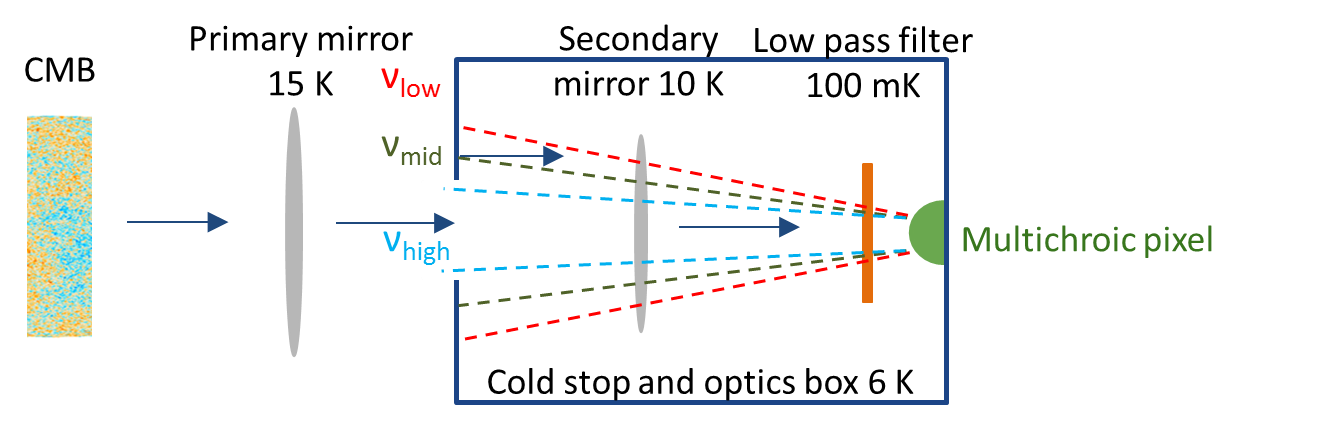
\includegraphics[height=5cm]{load_calc_MCP.png}
%\end{tabular}
\end{center}
\caption[load] { \label{fig:load} 
Schematic representation of the prediction of optical load.  Power emitted by each element is modified by the efficiency of the following elements 
and added to the total expected load.  The multichroic pixel illuminates the stop differently for each of the three bands.
}
\end{figure} 
%

For PICO, the CMB and stop dominate the optical loading as shown in Figure~\ref{fig:popt}.  %at low frequencies while and mirror emission 
% stop is ~1/3 of the load for 0.68 bands. 
%is the majority above 460~GHz due to their differing temperatures, see Figure~\ref{fig:popt}. 
The jumps in load between neighboring bands, seen in Figure~\ref{fig:popt} around 70 and 200~GHz, are due to $\eta_{stop}$ changing with frequency 
which is a consequence of using MCPs.  
The MCP angular beam width is dependent on the wavelength and pixel diameter\cite{suzuki2013_thesis},
\begin{equation}
\label{eq:mcp_beam}
\theta_{1/e^2} = \frac{2.95 \lambda}{\pi D_{px}}. 
\end{equation} 
The edge taper, T$_e$, of the middle frequency band in each pixel is chosen to be 10~dB. For the upper and lower bands T$_e$ is calculated using 
Equation~\ref{eq:mcp_beam}. This changing illumination of the stop is shown schematically by the dashed rays in Figure~\ref{fig:load}. 
For each MCP, A-H, T$_e$ is 4.8, 10, and 20.7~dB for the lower, middle, and upper bands, respectively.  These 
edge tapers correspond to $\eta_{stop}$ of 0.68, 0.90, and 0.99.
% meaning 32\% of the lowest band's throughput couples to the cold stop while only 1\% of the high frequency band's throughput copules to the stop.  
The changing $\eta_{stop}$ has three main effects; uneven optical load between bands, varying NEP to noise equivalent temperture (NET) conversion 
between bands, and telescope beam size not scaling smoothly with $\lambda$.

\begin{figure} [ht]
\begin{center}
\begin{tabular}{ccc} %% tabular useful for creating an array of images 
%\includegraphics[height=8cm]{P_optical.png}
\hspace{-1.4cm} 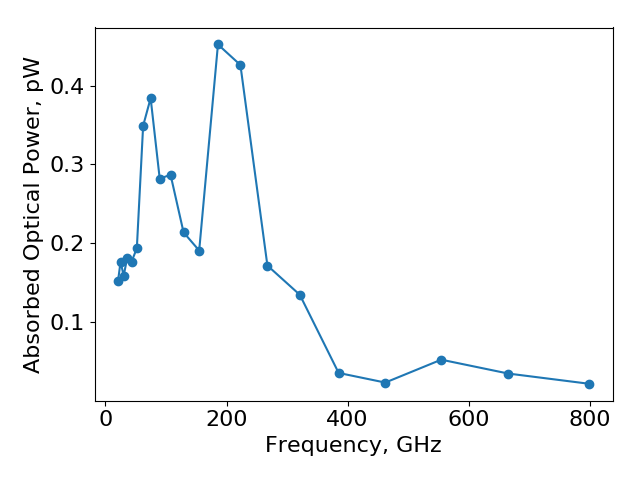
\includegraphics[height=4.9cm]{system_Popt.png} & \hspace{-0.7cm} 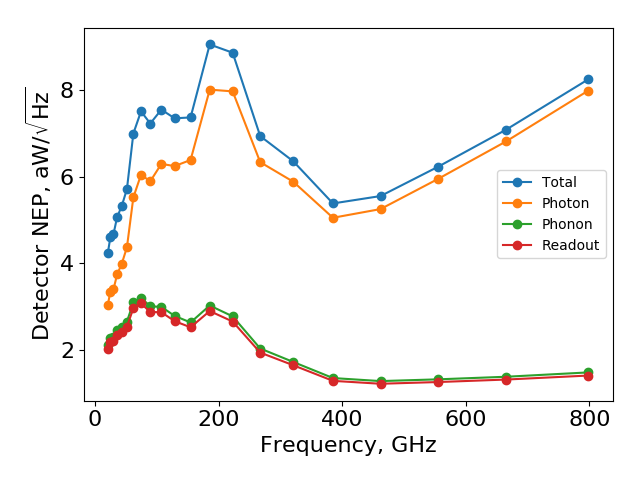
\includegraphics[height=4.9cm]{system_NEP.png} &\hspace{-0.7cm}  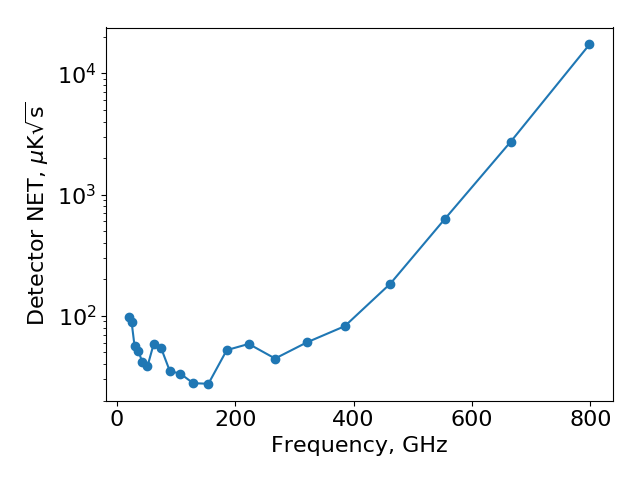
\includegraphics[height=4.9cm]{system_NET.png} 
\end{tabular}
\end{center}
\caption{ \label{fig:popt} \label{fig:noise} \label{fig:net} 
Left: Expected optical loads for single polarization PICO bolometers. 
Center: Breakdown of NEP across the PICO frequency range.  Photon noise dominates even at the lowest frequencies. 
Right: Single detector NET, temperature sensitivity,  across the PICO bands. %\comr{could add CORE NETs here for comparison. could add zoom around 150 GHz.}
}
\end{figure} 

%From $P_{abs}$ we calculate the TES bolometer properties for each band.  
%We assume a safety factor of 2, $P_{sat}/P_{abs}=2$; $P_{sat}$ is the 
%saturation power of the bolometer.  The PICO focal plane temperature, $T_o$, of 100~mK sets an optimal superconducting transition temperature, 
%$T_c$, of 187~mK.  We assume thermal conductivity scales as a power law, $G \propto T^n$,  with $n=2$.  The required thermal conductivity for 
%a given bolometer is set by the $P_{sat}$,
%any need to cite power law, G \propto T^n, assumption?
%\begin{equation}
%\label{eq:G}
%G = \frac{P_{sat}}{T_c} (n+1) \frac{1}{1-\left({T_o}{T_c}\right)^{n+1} }. 
%\end{equation} 
%\comr{need to say anything about C? tau? no real effect for FDM. if tau too long does matter for TDM. need to look in more detail. Roger assumed C = 1 pJ/K }

We consider four noise sources per bolometer; photon, phonon, TES Johnson, and readout. 
Photon noise depends on the absorbed power\cite{richards1994}, 
\begin{equation}
\label{eq:photon}
NEP_{\gamma}^2 = \int\limits_{band} 2h\nu p_{\nu} \, d\nu + 2\xi \int\limits_{band} p_{\nu}^2 \,  d\nu,
\end{equation} 
where $p_{\nu}$ is the power spectral density for a single polarization absorbed at the bolometer and $\xi$ is the fraction of correlated Bose 
photon noise. The extra factor of 2 in the Bose noise term is because we use single polarization bolometers.  
%
%
From $P_{abs}$ we calculate the TES bolometer properties and phonon noise.\cite{mather1982}  
%The second largest noise term is phonon noise\cite{mather1982} in the thermal connection to $T_o$,
%\begin{equation}
%\label{eq:phonon}
%NEP_{phonon}^2 = 4 \gamma k_b T_c^2 G,
%\end{equation} 
%where $\gamma$ is a unitless factor depending on $T_o$, $T_c$, and $n$. For PICO $\gamma=0.5$.
The last noise term intrinsic to the bolometer is the TES Johnson noise. All noise sources in the cold and warm readout 
electronics are lumped under the readout term.  The NEP for each noise source is shown in Figure~\ref{fig:noise}.
% something about the detailed readout model?  or in results?


% useful??
%\begin{equation} 
%\begin{split}
%\label{eq:readout}
%NEP_{readout}^2 &\propto V_{bias}^2 \propto  P_{e}, \text{ and}\\
%P_{e} &= P_{sat} - P_{abs}.
%\end{gather}
%\end{split}
%\end{equation}
%This neglects the details of our readout noise models, but is an illustrative approximation usefull for this paper.
% True for both. basically conversion of current noise to power.

% commentary.
\subsubsection{Results}  % not the best word to distinguish these two subsubsections.

%  RESULTS
For PICO, photon noise dominates at all frequencies as shown in Figure~\ref{fig:noise}. Bose noise is most significant 
at lower frequencies with NEP$_{Bose}$/NEP$_{Poisson}= 1.5 $ in the lowest band.  However, Poisson noise increases as 
$\sqrt{\nu}$, equalling Bose noise at 30~GHz and dominating at higher bands; NEP$_{Bose}$/NEP$_{Poisson} <10\%$ at 321~GHz. 
% this is NEP/NEP NOT squared.  Squared is 2.2 at 21 GHz and 0.01 at 321. < 10 at 129 GHz.  in NEP to NEP bose = poisson at 30 GHz
Phonon noise is the second most significant source, NEP$_{phonon}$/NEP$_{photon}$ ranges from 65\% at 21~GHz 
to 19\% at 799~GHz. 

For TDM readout phonon and readout noise are roughly equal, with TES Johnson noise being insignificant.  We also modeled 
FDM readout.  For FDM the TES Johnson noise is higher, 2/3 of the readout NEP, but the readout 
noise is lower.  Comparing the combinined Johnson and readout NEPs for TDM and FDM we find essentially indentical performance 
with total noise differing by less than 3\% across all bands.  For either system we require a focal plane temperature, $T_o$, of 
100~mK and a bolometer safety factor of 2 to remain photon noise dominated at the lowest bands.

The primary driver of noise levels is the optical load.  The combination of the CMB and aperture stop make up the majority of the load in all bands.
The load from the mirrors is greatest at 799~GHz where it is 90\% of that from the CMB and stop. The CMB provides more than half the load 
in the middle and upper bands of the multi-chroic pixels, but the stop dominates the load in the lowest band of each pixel.  Load from the 
stop in the lowest band of each pixel ranges from 1.2$\times$ the CMB load at 21~GHz to a maximum of 4.7$\times$ the CMB load at 223~GHz. 
%Two options to mitigate this extra load are a colder stop or more aggresive edge taper.


% RESULTS 
% Readout noise depends on the assumption of FDM or TDM readout and includes all remaining noise sources, the Johnson noise of the TES as well as 
% all components not intrinsic to the bolometers.  
% For both multiplexing schemes NEP$_{readout}$ is dominated by the SQUID amplifier with moderate contributions from various resistors 
% and amplifiers in the readout chain. We calculate noise for both FDM and TDM systems, though TDM is the current baseline, and find both to 
% be below both photon and phonon 
% noise for all bands.  Both systems give similar noise levels, with total noise differing by less than 3\% in all bands.
%  which is below the fidelity of the current study. 
% Some thought has been put into optimizing the readout systems for space, but since the expected noise is already sufficiently low this was not pursued 
% in detail. 
% For TDM and FDM the noise primarily scales with TES bias voltage which depends on the electrical power needed to operate the TES, 

%discussion of primary scalings and drivers? Popt does it all. choices like 100 mK and P/P = 2.
% The noise breakdown in Figure~\ref{fig:noise} drives various aspects of the PICO design. Since photon noise dominates at all frequencies and 
% photon noise scales with $\sqrt{P_{abs}}$, Equation~\ref{eq:photon}, the primary driver of noise is optical load.   The second largest source 
% of noise is phonon noise.  Combining
% Equations~\ref{eq:G} and~\ref{eq:phonon} we see $NEP_{phonon}$ scales with $\sqrt{T_C}$ and $\sqrt{P_{sat}}$.  Cooling the focal plane to 100~mK 
% reduces $T_c$ since $T_c \propto T_o$.  The saturation power depends on the choice of safety factor, $P_{sat}/P_{abs}$, as well as on optical load.  
% We choose safety factor of two to lower noise, while providing margin for unexpected loads or variations in $G$ of the fabricated 
% bolometers. Readout noise scales with $\sqrt{P_{sat} - P_{abs}}$, Equation~\ref{eq:readout}, which is reduced by reducing the safety factor or $P_{abs}$.  
% From this analysis we see that all noise sources depend on $P_{abs}$, either directly or through how load drives bolometer properties.  
% Therefore the 
% most straightforward way to reduce noise is to limit all optical loads other than the CMB.  This motivates the simple, few element telescope we 
% have designed with the aperture stop and secondary mirror actively cooled to reduce excess load and photon noise. 

\subsection{Combined  array noise}

Using single detector NEPs from Section~\ref{sec:det_noise} and the detector counts from Section~\ref{sec:focalplane} we 
calculate the combined NEP of the detector array for each band.  Generally, combining detectors simply reduces noise by $\sqrt{N}$.  The one 
exception is Bose photon noise. For the lowest band of each MCP the pixels oversample the PSF, pixel spacing is $0.4$F$\lambda$, resulting in correlated 
Bose noise bewteen pixels.  Accounting for this effect gives a 26\% increase in the combined array $NEP$ of the lowest band, 21~GHz, and only 
a 0.003\% increase in the highest band, 799~GHz.  

From the array $NEP$ we convert to $NET$ per band,
\begin{equation}
\label{eq:NET}
NET = \frac{NEP}{\sqrt{2} \, \eta_{opt} \int\limits_{band}\frac{dp_{\nu}}{dT}\Bigr|_{T_{CMB}} d\nu }.
\end{equation} 
The $\eta_{opt}$ term contributes to the `jumps' in $NET$ seen in Figure~\ref{fig:net} since $\eta_{opt}$ varies band to band.  
%We use CMB temperature units for all bands, even though this isn't particularly suitable for the highest bands, because the CMB is the most stringent requirement on sensitivity.

All the above calculations have been for sensitivity to temperature and are given in Table~\ref{tab:noise}.  Assuming evenly weighted observations 
of the full sky and 5 years observing at 95\% efficiency we calculate full mission map sensitivities in polarization; final column in Table~\ref{tab:noise}.
Combining all bands gives a total CMB map depth for the entire PICO mission of 0.62~$\mu$K$_{CMB}$-arcmin.

\begin{table}[ht]
\centering
\caption{PICO frequency channels and noise. }
\label{tab:noise}
\begin{tabular}{|c|c|c|c|c|c|c|c|}
\hline
Pixel  & Band  & FWHM   & Bolometer NEP & Bolometer NET        & N$_{bolo}$ & Array NET            & Polarization map depth  \\
Type   & GHz   & arcmin & aW/$\sqrt{Hz}$ & $\mu$K$_{CMB}\sqrt{s}$ &           & $\mu$K$_{CMB}\sqrt{s}$ & $\mu$K$_{CMB}$-arcmin      \\ \hline
A     & 21  & 38.4 & 4.89  & 112.2   & 120   & 12.9  & 18.2  \\
B     & 25  & 32.0 & 5.33  & 103.0   & 200   & 9.07   & 12.8  \\
A     & 30  & 28.3 & 4.92  & 59.4    & 120   & 5.60   & 7.88   \\
B     & 36  & 23.6 & 5.36  & 54.4    & 200   & 3.96   & 5.58   \\
A     & 43  & 22.2 & 5.33  & 41.7    & 120   & 3.80   & 5.36   \\
B     & 52  & 18.4 & 5.73  & 38.4    & 200   & 2.71   & 3.82   \\
C     & 62  & 12.8 & 8.29  & 69.2    & 732   & 2.97   & 4.19   \\
D     & 75  & 10.7 & 8.98  & 65.4    & 1020  & 2.34   & 3.29   \\
C     & 90  & 9.5  & 7.76  & 37.7    & 732   & 1.41   & 1.99   \\
D     & 108 & 7.9  & 8.18  & 36.2    & 1020  & 1.15   & 1.61   \\
C     & 129 & 7.4  & 7.35  & 27.8    & 732   & 1.03   & 1.45   \\
D     & 155 & 6.2  & 7.36  & 27.5    & 1020  & 0.86   & 1.21   \\
E     & 186 & 4.3  & 12.30 & 70.8    & 960   & 2.39   & 3.36   \\
F     & 223 & 3.6  & 12.70 & 84.2    & 900   & 2.89   & 4.07   \\
E     & 268 & 3.2  & 8.55  & 54.8    & 960   & 1.77   & 2.49   \\
F     & 321 & 2.6  & 8.16  & 77.6    & 900   & 2.59   & 3.64   \\
E     & 385 & 2.5  & 4.54  & 69.1    & 960   & 2.23   & 3.14   \\
F     & 462 & 2.1  & 4.00  & 132.6   & 900   & 4.42   & 6.22   \\
G     & 555 & 1.5  & 6.47  & 657.8   & 440   & 31.4  & 44.1  \\
H     & 666 & 1.3  & 5.74  & 2212    & 400   & 111 & 156 \\
I     & 799 & 1.1  & 4.97  & 10430   & 360   & 550 & 774 \\ 
\hline
Total &     &      &       &         & 12996 & 0.44   & 0.62  \\
\hline
\end{tabular}
\end{table}
%https://www.tablesgenerator.com/


\section{CONCLUSIONS/SUMMARY}

The PICO optical system is a simple two mirror Open Dragone which we numerically optimized to maximize the DLFOV.  The addition of a 
cold aperture stop and cold mirrors minimize optical load and reduce noise.  The focal plane takes advantage of the large DLFOV and MCP 
technology to implement 12996 polarization sensitive detectors in 21 bands from 21-799~GHz.  When combining all bands, our instrument 
noise model predicts full mission polarization map depth of 0.62~$\mu$K$_{CMB}$-arcmin.


% \begin{itemize}
% \item Total full sky map sensitivity, compare to Planck, LB, and S4? or do so in intro?
% \end{itemize}
% simple telescope. low noise? low systematics? - systematics not discussed elsewhere (yet)


% some of this phrasing here.
% From this analysis we see that all noise sources depend on $P_{abs}$, either directly or through how load drives bolometer properties.  
% Therefore the 
% most straightforward way to reduce noise is to limit all optical loads other than the CMB.  This motivates the simple, few element telescope we 
% have designed with the aperture stop and secondary mirror actively cooled to reduce excess load and photon noise. 


\section{ACKNOWLEDGEMENTS}

This Probe mission concept study is funded by NASA grant xxxxxxxx.  Gianfranco de Zotti acknowledges financial support from the ASI/University of
Roma--Tor Vergata agreement n.\; 2016-24-H.0 for study activities of the Italian cosmology community. Jacques
Delabrouille acknowledges financial support from PNCG for participating to the PICO study.


\bibliographystyle{spiebib} % makes bibtex use spiebib.bst
\bibliography{refs} % bibliography data in refs.bib


\end{document} 








% below is template guidelines to be deleted.

Begin the Introduction below the Keywords. The manuscript should not have headers, footers, or page numbers. It should be in a one-column format. References are often noted in the text and cited at the end of the paper.

\begin{table}[ht]
\caption{Fonts sizes to be used for various parts of the manuscript.  Table captions should be centered above the table.  When the caption is too long to fit on one line, it should be justified to the right and left margins of the body of the text.} 
\label{tab:fonts}
\begin{center}       
\begin{tabular}{|l|l|} %% this creates two columns
%% |l|l| to left justify each column entry
%% |c|c| to center each column entry
%% use of \rule[]{}{} below opens up each row
\hline
\rule[-1ex]{0pt}{3.5ex}  Article title & 16 pt., bold, centered  \\
\hline
\rule[-1ex]{0pt}{3.5ex}  Author names and affiliations & 12 pt., normal, centered   \\
\hline
\rule[-1ex]{0pt}{3.5ex}  Keywords & 10 pt., normal, left justified   \\
\hline
\rule[-1ex]{0pt}{3.5ex}  Abstract Title & 11 pt., bold, centered   \\
\hline
\rule[-1ex]{0pt}{3.5ex}  Abstract body text & 10 pt., normal, justified   \\
\hline
\rule[-1ex]{0pt}{3.5ex}  Section heading & 11 pt., bold, centered (all caps)  \\
\hline
\rule[-1ex]{0pt}{3.5ex}  Subsection heading & 11 pt., bold, left justified  \\
\hline
\rule[-1ex]{0pt}{3.5ex}  Sub-subsection heading & 10 pt., bold, left justified  \\
\hline
\rule[-1ex]{0pt}{3.5ex}  Normal text & 10 pt., normal, justified  \\
\hline
\rule[-1ex]{0pt}{3.5ex}  Figure and table captions & \, 9 pt., normal \\
\hline
\rule[-1ex]{0pt}{3.5ex}  Footnote & \, 9 pt., normal \\
\hline 
\rule[-1ex]{0pt}{3.5ex}  Reference Heading & 11 pt., bold, centered   \\
\hline
\rule[-1ex]{0pt}{3.5ex}  Reference Listing & 10 pt., normal, justified   \\
\hline
\end{tabular}
\end{center}
\end{table} 

\begin{table}[ht]
\caption{Margins and print area specifications.} 
\label{tab:Paper Margins}
\begin{center}       
\begin{tabular}{|l|l|l|} 
\hline
\rule[-1ex]{0pt}{3.5ex}  Margin & A4 & Letter  \\
\hline
\rule[-1ex]{0pt}{3.5ex}  Top margin & 2.54 cm & 1.0 in.   \\
\hline
\rule[-1ex]{0pt}{3.5ex}  Bottom margin & 4.94 cm & 1.25 in.  \\
\hline
\rule[-1ex]{0pt}{3.5ex}  Left, right margin & 1.925 cm & .875 in.  \\
\hline
\rule[-1ex]{0pt}{3.5ex}  Printable area & 17.15 x 22.23 cm & 6.75 x 8.75 in.  \\
\hline 
\end{tabular}
\end{center}
\end{table}

LaTeX margins are related to the document's paper size. The paper size is by default set to USA letter paper. To format a document for A4 paper, the first line of this LaTeX source file should be changed to \verb|\documentclass[a4paper]{spie}|.   

Authors are encouraged to follow the principles of sound technical writing, as described in Refs.~\citenum{Alred03} and \citenum{Perelman97}, for example.  Many aspects of technical writing are addressed in the {\em AIP Style Manual}, published by the American Institute of Physics.  It is available on line at \url{https://publishing.aip.org/authors}. A spelling checker is helpful for finding misspelled words. 

An author may use this LaTeX source file as a template by substituting his/her own text in each field.  This document is not meant to be a complete guide on how to use LaTeX.  For that, please see the list of references at \url{http://latex-project.org/guides/} and for an online introduction to LaTeX please see \citenum{Lees-Miller-LaTeX-course-1}. 

\section{FORMATTING OF MANUSCRIPT COMPONENTS}

This section describes the normal structure of a manuscript and how each part should be handled.  The appropriate vertical spacing between various parts of this document is achieved in LaTeX through the proper use of defined constructs, such as \verb|\section{}|.  In LaTeX, paragraphs are separated by blank lines in the source file. 

At times it may be desired, for formatting reasons, to break a line without starting a new paragraph.  This situation may occur, for example, when formatting the article title, author information, or section headings.  Line breaks are inserted in LaTeX by entering \verb|\\| or \verb|\linebreak| in the LaTeX source file at the desired location.  

\subsection{Title and Author Information}
\label{sec:title}

The article title appears centered at the top of the first page.  The title font is 16 point, bold.  The rules for capitalizing the title are the same as for sentences; only the first word, proper nouns, and acronyms should be capitalized.  Avoid using acronyms in the title.  Keep in mind that people outside your area of expertise might read your article. At the first occurrence of an acronym, spell it out, followed by the acronym in parentheses, e.g., noise power spectrum (NPS). 

The author list is in 12-pt. regular, centered. Omit titles and degrees such as Dr., Prof., Ph.D., etc. The list of affiliations follows the author list. Each author's affiliation should be clearly noted. Superscripts may be used to identify the correspondence between the authors and their respective affiliations.  Further author information, such as e-mail address, complete postal address, and web-site location, may be provided in a footnote by using \verb|\authorinfo{}|, as demonstrated above.

\subsection{Abstract and Keywords}
The title and author information is immediately followed by the Abstract. The Abstract should concisely summarize the key findings of the paper.  It should consist of a single paragraph containing no more than 250 words.  The Abstract does not have a section number.  A list of up to eight keywords should immediately follow the Abstract after a blank line.  These keywords will be included in a searchable database at SPIE.

\subsection{Body of Paper}
The body of the paper consists of numbered sections that present the main findings.  These sections should be organized to best present the material.  See Sec.~\ref{sec:sections} for formatting instructions.

\subsection{Appendices}
Auxiliary material that is best left out of the main body of the paper, for example, derivations of equations, proofs of theorems, and details of algorithms, may be included in appendices.  Appendices are enumerated with uppercase Latin letters in alphabetic order, and appear just before the Acknowledgments and References. Appendix~\ref{sec:misc} contains more about formatting equations and theorems.

\subsection{Acknowledgments}
In the Acknowledgments section, appearing just before the References, the authors may credit others for their guidance or help.  Also, funding sources may be stated.  The Acknowledgments section does not have a section number.

\subsection{References}
SPIE is able to display the references section of your paper in the SPIE Digital Library, complete with links to referenced journal articles, proceedings papers, and books, when available. This added feature will bring more readers to your paper and improve the usefulness of the SPIE Digital Library for all researchers. The References section does not have a section number.  The references are numbered in the order in which they are cited.  Examples of the format to be followed are given at the end of this document.  

The reference list at the end of this document is created using BibTeX, which looks through the file {\ttfamily report.bib} for the entries cited in the LaTeX source file.  The format of the reference list is determined by the bibliography style file {\ttfamily spiebib.bst}, as specified in the \verb|\bibliographystyle{spiebib}| command.  Alternatively, the references may be directly formatted in the LaTeX source file.

For books\cite{Lamport94,Alred03,Goossens97}, the listing includes the list of authors, book title, publisher, city, page or chapter numbers, and year of publication.  A reference to a journal article\cite{Metropolis53} includes the author list, title of the article (in quotes), journal name (in italics, properly abbreviated), volume number (in bold), inclusive page numbers, and year.  By convention\cite{Lamport94}, article titles are capitalized as described in Sec.~\ref{sec:title}.  A reference to a proceedings paper or a chapter in an edited book\cite{Gull89a} includes the author list, title of the article (in quotes), volume or series title (in italics), volume number (in bold), if applicable, inclusive page numbers, publisher, city, and year.  References to an article in the SPIE Proceedings may include the conference name (in italics), as shown in Ref.~\citenum{Hanson93c}. For websites\cite{Lees-Miller-LaTeX-course-1} the listing includes the list of authors, title of the article (in quotes), website name, article date, website address either enclosed in chevron symbols ('\(<\)' and '\(>\)'),  underlined or linked, and the date the website was accessed. 

If you use this formatting, your references will link your manuscript to other research papers that are in the CrossRef system. Exact punctuation is required for the automated linking to be successful. 

Citations to the references are made using superscript numerals, as demonstrated in the above paragraph.  One may also directly refer to a reference within the text, e.g., ``as shown in Ref.~\citenum{Metropolis53} ...''

\subsection{Footnotes}
Footnotes\footnote{Footnotes are indicated as superscript symbols to avoid confusion with citations.} may be used to provide auxiliary information that doesn't need to appear in the text, e.g., to explain measurement units.  They should be used sparingly, however.  

Only nine footnote symbols are available in LaTeX. If you have more than nine footnotes, you will need to restart the sequence using the command  \verb|\footnote[1]{Your footnote text goes here.}|. If you don't, LaTeX will provide the error message {\ttfamily Counter too large.}, followed by the offending footnote command.

\section{SECTION FORMATTING}
\label{sec:sections}

Section headings are centered and formatted completely in uppercase 11-point bold font.  Sections should be numbered sequentially, starting with the first section after the Abstract.  The heading starts with the section number, followed by a period.  In LaTeX, a new section is created with the \verb|\section{}| command, which automatically numbers the sections.

Paragraphs that immediately follow a section heading are leading paragraphs and should not be indented, according to standard publishing style\cite{Lamport94}.  The same goes for leading paragraphs of subsections and sub-subsections.  Subsequent paragraphs are standard paragraphs, with 14-pt.\ (5 mm) indentation.  An extra half-line space should be inserted between paragraphs.  In LaTeX, this spacing is specified by the parameter \verb|\parskip|, which is set in {\ttfamily spie.cls}.  Indentation of the first line of a paragraph may be avoided by starting it with \verb|\noindent|.
 
\subsection{Subsection Attributes}

The subsection heading is left justified and set in 11-point, bold font.  Capitalization rules are the same as those for book titles.  The first word of a subsection heading is capitalized.  The remaining words are also capitalized, except for minor words with fewer than four letters, such as articles (a, an, and the), short prepositions (of, at, by, for, in, etc.), and short conjunctions (and, or, as, but, etc.).  Subsection numbers consist of the section number, followed by a period, and the subsection number within that section.  

\subsubsection{Sub-subsection attributes}
The sub-subsection heading is left justified and its font is 10 point, bold.  Capitalize as for sentences.  The first word of a sub-subsection heading is capitalized.  The rest of the heading is not capitalized, except for acronyms and proper names.  

\section{FIGURES AND TABLES}

Figures are numbered in the order of their first citation.  They should appear in numerical order and on or after the same page as their first reference in the text.  Alternatively, all figures may be placed at the end of the manuscript, that is, after the Reference section.  It is preferable to have figures appear at the top or bottom of the page.  Figures, along with their captions, should be separated from the main text by at least 0.2 in.\ or 5 mm.  

Figure captions are centered below the figure or graph.  Figure captions start with the figure number in 9-point bold font, followed by a period; the text is in 9-point normal font; for example, ``{\footnotesize{Figure 3.}  Original image...}''.  See Fig.~\ref{fig:example} for an example of a figure caption.  When the caption is too long to fit on one line, it should be justified to the right and left margins of the body of the text.  

Tables are handled identically to figures, except that their captions appear above the table. 

% Note: If compiling with LaTeX+dvipdf, please ensure images generated from 
% other software packages have their bounding boxes set correctly.
   \begin{figure} [ht]
   \begin{center}
   \begin{tabular}{c} %% tabular useful for creating an array of images 
   \includegraphics[height=5cm]{mcr3b.eps}
   \end{tabular}
   \end{center}
   \caption[example] 
%>>>> use \label inside caption to get Fig. number with \ref{}
   { \label{fig:example} 
Figure captions are used to describe the figure and help the reader understand it's significance.  The caption should be centered underneath the figure and set in 9-point font.  It is preferable for figures and tables to be placed at the top or bottom of the page. LaTeX tends to adhere to this standard.}
   \end{figure} 

\section{MULTIMEDIA FIGURES - VIDEO AND AUDIO FILES}

Video and audio files can be included for publication. See Tab.~\ref{tab:Multimedia-Specifications} for the specifications for the mulitimedia files. Use a screenshot or another .jpg illustration for placement in the text. Use the file name to begin the caption. The text of the caption must end with the text ``http://dx.doi.org/doi.number.goes.here'' which tells the SPIE editor where to insert the hyperlink in the digital version of the manuscript. 

Here is a sample illustration and caption for a multimedia file:

   \begin{figure} [ht]
   \begin{center}
   \begin{tabular}{c} 
   \includegraphics[height=5cm]{MultimediaFigure.jpg}
	\end{tabular}
	\end{center}
   \caption[example] 
   { \label{fig:video-example} 
A label of “Video/Audio 1, 2, …” should appear at the beginning of the caption to indicate to which multimedia file it is linked . Include this text at the end of the caption: \url{http://dx.doi.org/doi.number.goes.here}}
   \end{figure} 
   
   \begin{table}[ht]
\caption{Information on video and audio files that must accompany a manuscript submission.} 
\label{tab:Multimedia-Specifications}
\begin{center}       
\begin{tabular}{|l|l|l|}
\hline
\rule[-1ex]{0pt}{3.5ex}  Item & Video & Audio  \\
\hline
\rule[-1ex]{0pt}{3.5ex}  File name & Video1, video2... & Audio1, audio2...   \\
\hline
\rule[-1ex]{0pt}{3.5ex}  Number of files & 0-10 & 0-10  \\
\hline
\rule[-1ex]{0pt}{3.5ex}  Size of each file & 5 MB & 5 MB  \\
\hline
\rule[-1ex]{0pt}{3.5ex}  File types accepted & .mpeg, .mov (Quicktime), .wmv (Windows Media Player) & .wav, .mp3  \\
\hline 
\end{tabular}
\end{center}
\end{table}

\appendix    %>>>> this command starts appendixes

\section{MISCELLANEOUS FORMATTING DETAILS}
\label{sec:misc}

It is often useful to refer back (or forward) to other sections in the article.  Such references are made by section number.  When a section reference starts a sentence, Section is spelled out; otherwise use its abbreviation, for example, ``In Sec.~2 we showed...'' or ``Section~2.1 contained a description...''.  References to figures, tables, and theorems are handled the same way.

\subsection{Formatting Equations}
Equations may appear in line with the text, if they are simple, short, and not of major importance; e.g., $\beta = b/r$.  Important equations appear on their own line.  Such equations are centered.  For example, ``The expression for the field of view is
\begin{equation}
\label{eq:fov}
2 a = \frac{(b + 1)}{3c} \, ,
\end{equation}
where $a$ is the ...'' Principal equations are numbered, with the equation number placed within parentheses and right justified.  

Equations are considered to be part of a sentence and should be punctuated accordingly. In the above example, a comma follows the equation because the next line is a subordinate clause.  If the equation ends the sentence, a period should follow the equation.  The line following an equation should not be indented unless it is meant to start a new paragraph.  Indentation after an equation is avoided in LaTeX by not leaving a blank line between the equation and the subsequent text.

References to equations include the equation number in parentheses, for example, ``Equation~(\ref{eq:fov}) shows ...'' or ``Combining Eqs.~(2) and (3), we obtain...''  Using a tilde in the LaTeX source file between two characters avoids unwanted line breaks.

\subsection{Formatting Theorems}

To include theorems in a formal way, the theorem identification should appear in a 10-point, bold font, left justified and followed by a period.  The text of the theorem continues on the same line in normal, 10-point font.  For example, 

\noindent\textbf{Theorem 1.} For any unbiased estimator...

Formal statements of lemmas and algorithms receive a similar treatment.

\acknowledgments % equivalent to \section*{ACKNOWLEDGMENTS}       
 
This unnumbered section is used to identify those who have aided the authors in understanding or accomplishing the work presented and to acknowledge sources of funding.  

% References
